\documentclass[UTF8]{article}

\usepackage{ctex}
\usepackage{multicol}
\usepackage{geometry}
\usepackage{graphicx}
\usepackage{lmodern}
\usepackage{amsmath}
\usepackage{listings}
\usepackage{float}
\usepackage[table,xcdraw]{xcolor}
\lstset{language=Matlab}

\geometry{left=1cm, right=1cm, top=2cm, bottom=2cm}
\fontsize{5pt}{\baselineskip}\selectfont

\setlength\columnsep{1cm}

\title{神经网络第二次实验报告}
\author{谢涵 PB19071443}
\date{\today}

\begin{document}
\maketitle
\section{实验题目}
根据所学过的BP网络设计及改进方案设计实现模糊控制规则为
$T= int((e+ec)/2)$的模糊神经网络控制器,其中输入变量\emph{e}和\emph{ec}的
变化范围分别是:$e = int[-2, 2],\ ec = int[-2, 2]$。网络设计的目标误差为0.001。

\section{实验设计}
\subsection{输入、输出矢量}
输入矩阵:
\begin{equation}
	P=\left(
        \addtocounter{MaxMatrixCols}{25}
        \begin{matrix}
		-2 & -2 & -2 & -2 & -2 & -1 & -1 & -1 & -1 & -1 & 0  & 0  & 0 & 0 & 0 & 1  & 1  & 1 & 1 & 1 & 2  & 2  & 2 & 2 & 2 \\
		-2 & -1 & 0  & 1  & 2  & -2 & -1 & 0  & 1  & 2  & -2 & -1 & 0 & 1 & 2 & -2 & -1 & 0 & 1 & 2 & -2 & -1 & 0 & 1 & 2
	\end{matrix}\nonumber
	\right)
\end{equation}
目标矩阵(取下整):
\begin{equation}
	T=\left(
	\begin{matrix}
		-2 & -2 & -1 & -1 & 0 & -2 & -1 & -1 & 0 & 0 & -1 & -1 & 0 & 0 & 1 & -1 & 0 & 0 & 1 & 1 & 0 & 0 & 1 & 1 & 2
	\end{matrix}\nonumber
	\right)
\end{equation}
\subsection{网络结构}
输入大小为$2\times 25$,输出大小为$1\times 25$,含有一个隐含层,一个输出层,层数为2:n:1
\begin{figure}[H]
\centering
	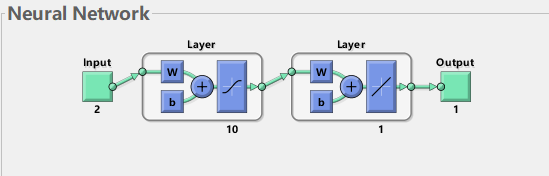
\includegraphics[width=0.6\textwidth]{image1.png}
    \caption[0.3\textwidth]{网络结构}
\end{figure}

\section{实验项目}
\subsection{S1大小对实验的影响}
\subsubsection{代码段}
\begin{lstlisting}
    P = [-2 -2 -2 -2 -2 -1 -1 -1 -1 -1  0  0 0 0 0  1  1 1 1 1  2  2 2 2 2;
        -2 -1  0  1  2 -2 -1  0  1  2 -2 -1 0 1 2 -2 -1 0 1 2 -2 -1 0 1 2];

    T = [-2 -2 -1 -1 0  -2 -1 -1  0  0 -1 -1 0 0 1 -1  0 0 1 1  0  0 1 1 2];

    S1 = 7;  % vary from 7 to 13
    [R, ~] = size(P);
    [S2, Q] = size(T);

    net = newff(minmax(P), [S1,1], {'tansig', 'purelin'}, 'traingd'); 
    % 初始化
    net.IW{1, 1} = rands(S1, R);
    net.b{1} = rands(S1, 1);
    net.LW{2, 1} = rands(S2, S1);
    net.b{2} = rands(S2, 1);

    net.trainParam.epochs = 10000;
    net.trainParam.lr = 0.03;
    net.trainParam.goal = 1e-3;

    [net,tr]= train(net, P, T, nnMATLAB); 
    Y = sim(net, P);
    sse_error = perform(net, T, Y);
    fprintf('SSE=%f\n', sse_error);
\end{lstlisting}
\subsubsection{实验结果}
取学习率为0.03,由于测试发现经过数万次训练后均未达到1e-3误差期望值,故均以10000次为max\_epochs
% \makeatletter\def\@captype{table}\makeatother
\begin{table}[H] \centering
    \begin{tabular}{ccccl}
    \rowcolor[HTML]{FFFFFF} 
    {\color[HTML]{333333} \textbf{S1}} & {\color[HTML]{333333} \textbf{时间/s}} & {\color[HTML]{333333} \textbf{训练次数}} & {\color[HTML]{333333} \textbf{SSE}} & {\color[HTML]{333333} \textbf{收敛速度}} \\
    \rowcolor[HTML]{FFFFFF} 
    {\color[HTML]{333333} 7} & {\color[HTML]{333333} 9} & {\color[HTML]{333333} 10000} & {\color[HTML]{333333} 0.0574} & {\color[HTML]{333333} 开始几步误差下降很快,此后快速变慢,此后下降极为缓慢} \\
    \rowcolor[HTML]{F8F8F8} 
    {\color[HTML]{333333} 8} & {\color[HTML]{333333} 9} & {\color[HTML]{333333} 10000} & {\color[HTML]{333333} 0.0575} & {\color[HTML]{333333} 开始几步误差下降很快,此后下降极为缓慢} \\
    \rowcolor[HTML]{FFFFFF} 
    {\color[HTML]{333333} 9} & {\color[HTML]{333333} 9} & {\color[HTML]{333333} 10000} & {\color[HTML]{333333} 0.0519} & {\color[HTML]{333333} 开始几步误差下降很快,此后下降极为缓慢} \\
    \rowcolor[HTML]{F8F8F8} 
    {\color[HTML]{333333} 10} & {\color[HTML]{333333} 9} & {\color[HTML]{333333} 10000} & {\color[HTML]{333333} 0.0215} & {\color[HTML]{333333} 开始几步误差下降很快,此后下降变缓但较为明显} \\
    \rowcolor[HTML]{FFFFFF} 
    {\color[HTML]{333333} 11} & {\color[HTML]{333333} 9} & {\color[HTML]{333333} 10000} & {\color[HTML]{333333} 0.0347} & {\color[HTML]{333333} 开始几步误差下降很快,此后下降变缓但较为明显} \\
    \rowcolor[HTML]{F8F8F8} 
    {\color[HTML]{333333} 12} & {\color[HTML]{333333} 9} & {\color[HTML]{333333} 10000} & {\color[HTML]{333333} 0.0584} & {\color[HTML]{333333} 开始几步误差下降很快,此后下降极为缓慢} \\
    \rowcolor[HTML]{FFFFFF} 
    {\color[HTML]{333333} 13} & {\color[HTML]{333333} 9} & {\color[HTML]{333333} 10000} & {\color[HTML]{333333} 0.0525} & {\color[HTML]{333333} 开始几步误差下降很快,此后下降极为缓慢}
    \end{tabular}
\caption[0.3\textwidth]{S1结果}
\end{table}
根据测试结果,可以发现在S1取值为10或11的时候效果最好,因此取$S1=10$
\subsection{取定S1,观察lr大小对实验的影响}
实验代码同3.1.1,修改如下:epoch=25000,取定S1=10,改变lr的值。每个lr值重复多次,取最有代表性的一次作为结果,见表2。\\
\begin{table}[] \caption[0.3\textwidth]{lr结果} \centering
    \begin{tabular}{cccc}
    \rowcolor[HTML]{FFFFFF} 
    {\color[HTML]{333333} \textbf{lr}} & {\color[HTML]{333333} \textbf{时间/s}} & {\color[HTML]{333333} \textbf{SSE}} & {\color[HTML]{333333} \textbf{稳定性}} \\
    \rowcolor[HTML]{FFFFFF} 
    {\color[HTML]{333333} 0.01} & {\color[HTML]{333333} 25} & {\color[HTML]{333333} 0.0344} & {\color[HTML]{333333} 急剧下降-几乎不下降,平滑} \\
    \rowcolor[HTML]{F8F8F8} 
    {\color[HTML]{333333} 0.02} & {\color[HTML]{333333} 25} & {\color[HTML]{333333} 0.0234} & {\color[HTML]{333333} 急剧下降-几乎不下降,平滑} \\
    \rowcolor[HTML]{FFFFFF} 
    {\color[HTML]{333333} 0.03} & {\color[HTML]{333333} 25} & {\color[HTML]{333333} 0.0148} & {\color[HTML]{333333} 急剧下降-速度变缓-几乎不下降,平滑} \\
    \rowcolor[HTML]{F8F8F8} 
    {\color[HTML]{333333} 0.04} & {\color[HTML]{333333} 25} & {\color[HTML]{333333} 0.00825} & {\color[HTML]{333333} 急剧下降-速度变缓-较快速下降,平滑} \\
    \rowcolor[HTML]{FFFFFF} 
    {\color[HTML]{333333} 0.05} & {\color[HTML]{333333} 25} & {\color[HTML]{333333} 0.00251} & {\color[HTML]{333333} 急剧下降-速度变缓-较快速下降,平滑} \\
    \rowcolor[HTML]{F8F8F8} 
    {\color[HTML]{333333} 0.06} & {\color[HTML]{333333} 24} & {\color[HTML]{333333} 0.00137} & {\color[HTML]{333333} 急剧下降-速度变缓-较快速下降,平滑} \\
    \rowcolor[HTML]{FFFFFF} 
    {\color[HTML]{333333} 0.07} & {\color[HTML]{333333} 23} & {\color[HTML]{333333} 0.001} & {\color[HTML]{333333} 急剧下降-快速下降,直至达到预期误差1e-3,迭代次数22789,平滑} \\
    \rowcolor[HTML]{F8F8F8} 
    {\color[HTML]{333333} 0.08} & {\color[HTML]{333333} 13} & {\color[HTML]{333333} 0.001} & {\color[HTML]{333333} 急剧下降-快速下降,直至达到预期误差1e-3,迭代次数14833,多次试验均平滑} \\
    \rowcolor[HTML]{FFFFFF} 
    {\color[HTML]{333333} 0.09} & {\color[HTML]{333333} 15} & {\color[HTML]{333333} 0.001} & {\color[HTML]{333333} \begin{tabular}[c]{@{}l@{}}急剧下降-快速下降,直至达到预期误差1e-3,迭代次数15020,有时出现波动,\\ 有时完全平缓\end{tabular}} \\
    \rowcolor[HTML]{F8F8F8} 
    {\color[HTML]{333333} 0.1} & {\color[HTML]{333333} 24} & {\color[HTML]{333333} 0.0194} & {\color[HTML]{333333} 急剧下降-速度变缓,中途出现许多细小的波动,平滑} \\
    \rowcolor[HTML]{FFFFFF} 
    {\color[HTML]{333333} 0.11} & {\color[HTML]{333333} 24} & {\color[HTML]{333333} 0.0139} & {\color[HTML]{333333} 急剧下降-速度变缓,但是中途出现了两个尖锐的波动,其余部分平滑} \\
    \rowcolor[HTML]{F8F8F8} 
    {\color[HTML]{333333} 0.12} & {\color[HTML]{333333} 18} & {\color[HTML]{333333} 0.001} & {\color[HTML]{333333} \begin{tabular}[c]{@{}l@{}}急剧下降-速度变缓,后半段出现密集连续的波动,波动逐步减小直至到达预期误差,\\ 迭代次数18864\end{tabular}} \\
    \rowcolor[HTML]{FFFFFF} 
    {\color[HTML]{333333} 0.13} & {\color[HTML]{333333} 20} & {\color[HTML]{333333} 0.001} & {\color[HTML]{333333} \begin{tabular}[c]{@{}l@{}}急剧下降-速度变缓,中途出现更多更尖锐的波动,波动逐步减小直至到达预期误差,\\ 迭代次数21639\end{tabular}} \\
    \rowcolor[HTML]{F8F8F8} 
    {\color[HTML]{333333} 0.3} & {\color[HTML]{333333} 28} & {\color[HTML]{333333} 0.00296} & {\color[HTML]{333333} \begin{tabular}[c]{@{}l@{}}出现密集连续的波动,在某个值附近反复升降而总体下降极为缓慢,25000次迭代 \\ 后仍未收敛 \end{tabular}} \\
\end{tabular}
\end{table}

可以发现在lr逐渐增大的过程中,首先收敛速度变快,但当lr特别大时会出现波动,
但仍会较快地达到预期误差。实验中效果最好的学习率为 $lr=0.08$

\subsection{取定S1和lr,固定学习率与自适应值学习率进行对比}
将学习方法改为'traingda',取初始lr=0.08,进行实验,得到结果,见表3。
\begin{table}[H] \caption[0.3\textwidth]{gda结果} \centering
\begin{tabular}{ccccc}
\rowcolor[HTML]{FFFFFF} 
{\color[HTML]{333333} \textbf{学习方法}} & {\color[HTML]{333333} \textbf{迭代次数}} & {\color[HTML]{333333} \textbf{时间/s}} & {\color[HTML]{333333} \textbf{SSE}} & {\color[HTML]{333333} \textbf{观察}} \\
gd & 14833 & 13 & 0.001 & \begin{tabular}[c]{@{}l@{}}急剧下降-快速下降,直至达到预期误差1e-3,迭代次数14833,多次\\ 试验均平滑\end{tabular} \\
\rowcolor[HTML]{FFFFFF} 
{\color[HTML]{333333} gda} & {\color[HTML]{333333} 12883} & {\color[HTML]{333333} 11} & {\color[HTML]{333333} 0.000999} & {\color[HTML]{333333} \begin{tabular}[c]{@{}l@{}}有密集的波动,总体以较快速度降至指定误差,波动符合gda学习法\\ 的特性\end{tabular}}
\end{tabular}
\end{table}

可以发现gda学习速率较快,虽然有震荡,但是能更快地收敛到给定误差内

\section{实验分析和实验结论}
\subsection{优化算法对比}
选定$S1=10, lr=0.08$,修改代码如下:
\begin{lstlisting}
    P = [-2 -2 -2 -2 -2 -1 -1 -1 -1 -1  0  0 0 0 0  1  1 1 1 1  2  2 2 2 2;
        -2 -1  0  1  2 -2 -1  0  1  2 -2 -1 0 1 2 -2 -1 0 1 2 -2 -1 0 1 2];

    T = [-2 -2 -1 -1 0  -2 -1 -1  0  0 -1 -1 0 0 1 -1  0 0 1 1  0  0 1 1 2];

    S1 = 10;
    [R, ~] = size(P);
    [S2, Q] = size(T);

    % ????为待选择的训练方法 
    net = newff(minmax(P), [S1,1], {'tansig', 'purelin'}, '????');

    % 初始化
    net.IW{1, 1} = rands(S1, R);
    net.b{1} = rands(S1, 1);
    net.LW{2, 1} = rands(S2, S1);
    net.b{2} = rands(S2, 1);

    % 打印初始权重
    net.IW{1, 1}
    net.b{1}
    net.LW{2, 1}
    net.b{2}

    net.trainParam.epochs = 25000;
    net.trainParam.lr = 0.08;
    net.trainParam.goal = 1e-3;
    % net.trainParam.mc = 0.9; % 如果选择附加动量法则使用这行代码

    [net,tr]= train(net, P, T, nnMATLAB); 
    Y = sim(net ,P);

    sse_error = perform(net, T, Y);
    fprintf('SSE=%f\n', sse_error);
    % 打印训练完毕后的权重
    net.IW{1, 1}
    net.b{1}
    net.LW{2, 1}
    net.b{2}

\end{lstlisting}
\subsubsection{标准梯度下降法gd}
训练次数:16251

训练前:
\begin{equation}
\nonumber
\begin{aligned}
    W_{11} = 
    \left(
    \begin{matrix}
        -0.5638 &  0.8182\\
        0.5447 &  0.1832\\
        -0.5439 & -0.3349\\
        -0.2583 &  0.7061\\
        0.7819 & -0.1152\\
        0.7128  & 0.8087\\
        -0.1951 & -0.9336\\
        -0.3640 &  0.0649\\
        0.2173 & 0.4330\\
        0.8204 & -0.6414\\
    \end{matrix}
    \right)
    \quad
    b_{1} = 
    \left(
    \begin{matrix}
        -0.3269\\
        -0.6246\\
        -0.3561\\
        -0.1923\\
            0.0971\\
        -0.9025\\
            0.1055\\
        -0.4504\\
        -0.5170\\
        -0.5137
    \end{matrix}
    \right)
    \quad
    W_{21}^T = 
    \left(
    \begin{matrix}
        -0.6917 \\  0.9128\\ 0.8713\\  0.6374\\ 0.4565\\ -0.6484\\-0.2793\\-0.6224 \\-0.9976 \\-0.3672
    \end{matrix}
    \right)
    \quad
    b_{2} = 
    \left(
    \begin{matrix}
        0.3992
    \end{matrix}
    \right)
\end{aligned}
\end{equation}

训练后:
\begin{equation}
\nonumber
\begin{aligned}
W_{11} = 
\left(
\begin{matrix}
    -1.7815 & 0.2940\\
    0.2629 & 0.3417\\
   -1.0599 & -1.3226\\
   -1.2449 & 1.1064\\
    1.7894 & -0.2905\\
    1.3699 & 1.4391\\
   -2.8287 & -2.5381\\
   -1.0009 & -0.8621\\
    0.5668 & -0.8834\\
    1.9805 & -0.9055
\end{matrix}
\right)
\quad
b_{1} = 
\left(
\begin{matrix}
    -0.2671\\
   -1.3431\\
   -2.5425\\
    0.5865\\
    0.8894\\
   -1.5661\\
   -1.3257\\
   -0.4214\\
   -0.5369\\
   -0.6297
\end{matrix}
\right)
\quad
W_{21}^T = 
\left(
\begin{matrix}
    1.1239\\1.2695\\ -1.1295 \\ 0.9885 \\ 0.8170 \\ 0.9766\\ -1.6034\\ 2.3424 \\ 0.6884 \\  0.9597
\end{matrix}
\right)
\quad
b_{2} = 
\left(
\begin{matrix}
    0.4768
\end{matrix}
\right)
\end{aligned}
\end{equation}
\begin{center}
$SSE = 0.001000$
\end{center}
\begin{figure}[H]
\centering
    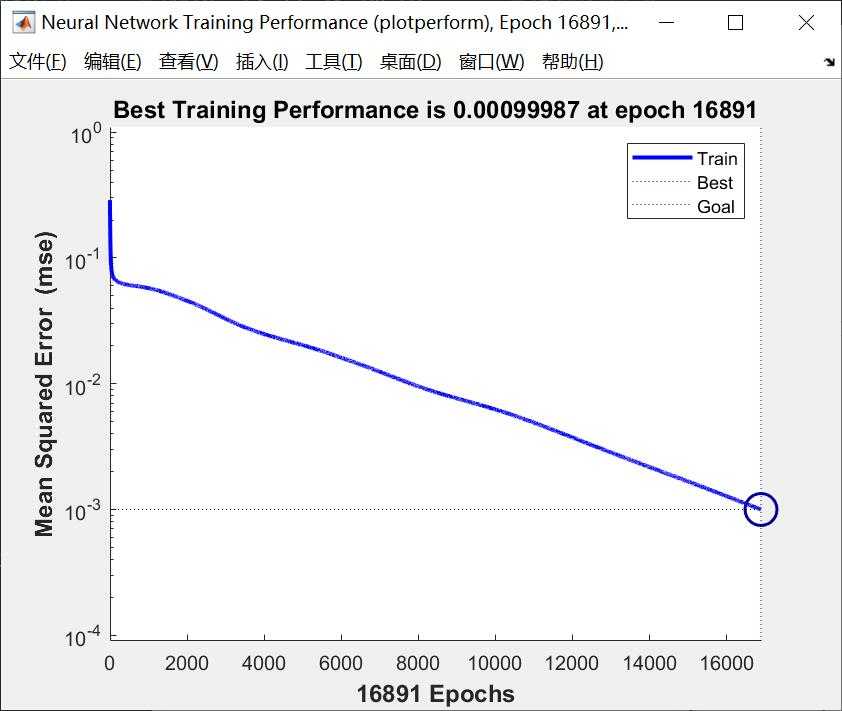
\includegraphics[width=0.55\textwidth]{gd.jpg}
    \caption[0.3\textwidth]{gd损失函数}
\end{figure}

\subsubsection{附加动量的BP算法,取动量因子mc=0.9}
训练次数:16891

训练前:
\begin{equation}
\nonumber
\begin{aligned}
    W_{11} = 
    \left(
    \begin{matrix}
        -0.4619& -0.6355\\
        0.3461 &  -0.8018\\
        -0.0450 &  -0.0205\\
        0.2474  & -0.6135\\
        -0.5271&    0.7918\\
        -0.6458  & -0.8018\\
        0.6593  & -0.9117\\
        0.5338  &  0.1146\\
        0.8690 &   0.5450\\
        -0.7842 &  -0.3761
    \end{matrix}
    \right)
    \quad
    b_{1} = 
    \left(
    \begin{matrix}
        -0.6420\\
        -0.3221\\
        -0.5797\\
        0.0203\\
        0.8127\\
        0.2578\\
        -0.7969\\
        -0.2183\\
        -0.8908\\
        0.0026
    \end{matrix}
    \right)
    \quad
    W_{21}^T = 
    \left(
    \begin{matrix}
        -0.1366 \\ 0.9951 \\ 0.6232 \\ -0.0287\\ 0.7889 \\-0.7249 \\-0.2200 \\ 0.8547 \\0.8350 \\0.4271
    \end{matrix}
    \right)
    \quad
    b_{2} = 
    \left(
    \begin{matrix}
        0.2367
    \end{matrix}
    \right)
\end{aligned}
\end{equation}

训练后:
\begin{equation}
\nonumber
\begin{aligned}
W_{11} = 
\left(
\begin{matrix}
    -0.9573 & -0.2569\\
    1.3049 & -1.2086\\
   -0.2774 &  0.5344\\
    1.0700 & -1.9800\\
   -0.7717 &  0.9733\\
   -1.2740 & -1.2264\\
    2.6109 & -2.8408\\
    0.2721 & -0.9573\\
    0.6979 & -0.1031\\
   -2.6447 & -2.6884
\end{matrix}
\right)
\quad
b_{1} = 
\left(
\begin{matrix}
    -1.7565\\
   -0.7089\\
   -1.4201\\
    1.1507\\
    1.3040\\
    0.7523\\
   -1.6655\\
    0.3968\\
   -1.6833\\
    1.5357
\end{matrix}
\right)
\quad
W_{21}^T = 
\left(
\begin{matrix}
    -0.7211\\ 2.6790\\  0.9172\\ -1.1196\\ 1.1644\\-2.2634\\-1.6824\\1.2569\\ 0.4637 \\ 1.4626
\end{matrix}
\right)
\quad
b_{2} = 
\left(
\begin{matrix}
    0.1742
\end{matrix}
\right)
\end{aligned}
\end{equation}
\begin{center}
$SSE = 0.001000$
\end{center}
\begin{figure}[H]
\centering
    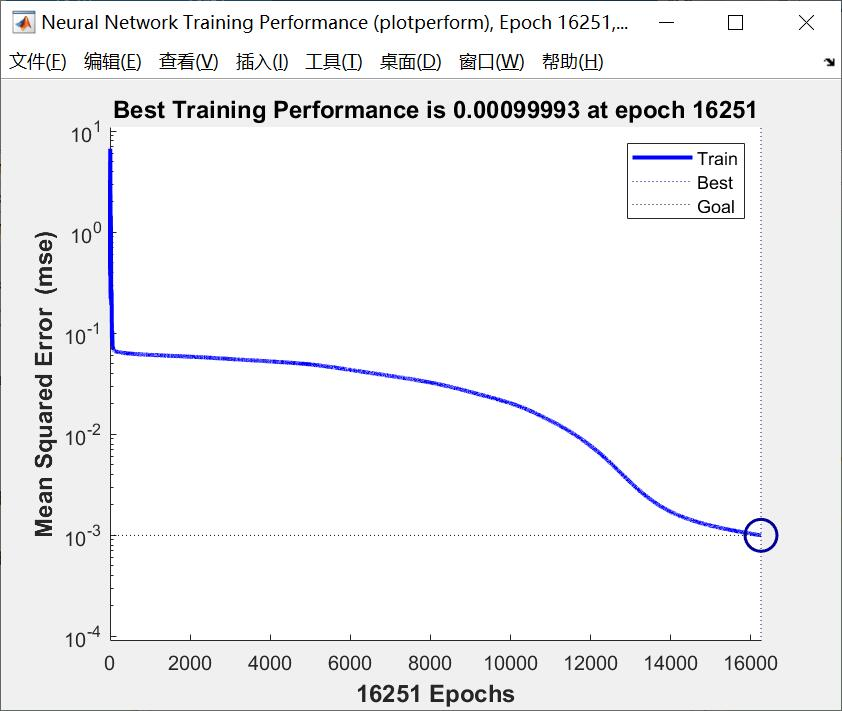
\includegraphics[width=0.4\textwidth]{gdm.jpg}
    \caption[0.3\textwidth]{gdm损失函数}
\end{figure}

\subsubsection{Levenberg-Marquardt法}
训练次数:39

训练前:
\begin{equation}
\nonumber
\begin{aligned}
    W_{11} = 
    \left(
    \begin{matrix}
        -0.7803 & 0.2786\\
   -0.7805 & -0.4893\\
   -0.4602 & -0.8227\\
    0.0493 &  0.6765\\
    0.9453 &  0.1694\\
    0.4208  & 0.8962\\
   -0.3763 & -0.8779\\
   -0.4171 &  0.1693\\
    0.7007 & -0.4298\\
    0.8233 &  0.6555
    \end{matrix}
    \right)
    \quad
    b_{1} = 
    \left(
    \begin{matrix}
        -0.6180\\
        -0.1149\\
        -0.2132\\
         0.6531\\
         0.3537\\
        -0.5848\\
        -0.3638\\
        -0.7324\\
         0.3429\\
         0.1420
    \end{matrix}
    \right)
    \quad
    W_{21}^T = 
    \left(
    \begin{matrix}
        -0.6605\\-0.7047\\ -0.0478 \\  0.8162\\ 0.1044 \\ -0.9341 \\-0.8923 \\  0.6101 \\ -0.0973\\-0.2347
    \end{matrix}
    \right)
    \quad
    b_{2} = 
    \left(
    \begin{matrix}
        0.5793
    \end{matrix}
    \right)
\end{aligned}
\end{equation}

训练后:
\begin{equation}
\nonumber
\begin{aligned}
W_{11} = 
\left(
\begin{matrix}
    0.4530  & 0.4104\\
   -0.7801 &  -0.8170\\
   -1.2386  & -1.2801\\
    1.2494  &  1.2425\\
    0.3602  &  0.3428\\
    3.5719  &  3.5260\\
   -0.8858  &  0.0796\\
   -0.7731  & -0.1004\\
    1.1326  &  0.0859\\
    1.2909  &  1.2316\\
\end{matrix}
\right)
\quad
b_{1} = 
\left(
\begin{matrix}
    -0.6978\\
    3.1564\\
    0.6007\\
    3.0192\\
    0.5527\\
   -1.7111\\
    0.8649\\
   -1.1725\\
    1.4703\\
   -0.6260\\
\end{matrix}
\right)
\quad
W_{21}^T = 
\left(
\begin{matrix}
    -1.7882 \\ -2.1195 \\  -2.8277  \\  1.6122   \\-2.2055  \\ -2.5057\\
   -0.1581 \\   0.7508 \\   0.5739 \\   2.3367
\end{matrix}
\right)
\quad
b_{2} = 
\left(
\begin{matrix}
    1.2189
\end{matrix}
\right)
\end{aligned}
\end{equation}
\begin{center}
$SSE = 0.000226$
\end{center}
\begin{figure}[H]
\centering
    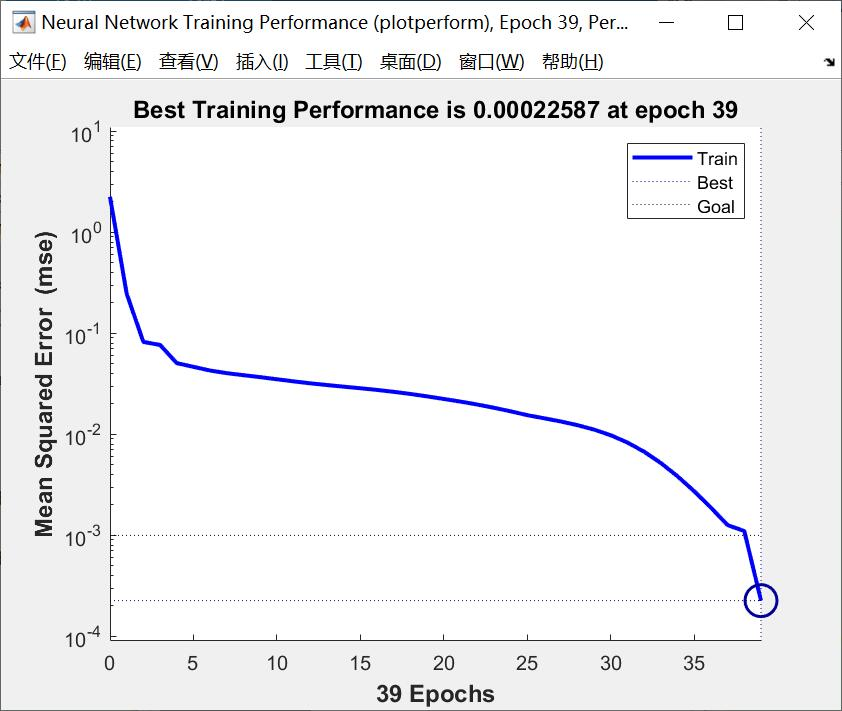
\includegraphics[width=0.4\textwidth]{lm.jpg}
    \caption[0.3\textwidth]{lm损失函数}
\end{figure}

\subsection{插值法验证}
对于前面取$S1=10, lr = 0.08$,用gd法已训练好的网络,差值范围为$-2:0.5:2$,进行差值测试如下
\subsubsection{测试代码}
\begin{lstlisting}
    % 样本插值测试
    P1 = zeros();
    T1 = zeros();
    step = 0.5;
    e1 = -2:step:2;
    ec1 = -2:step:2;
    [~, S] = size(e1);
    for i = 1:S
        for j = 1:S
            col = (i-1) * S + j;
            P1(1, col) = e1(i);
            P1(2, col) = ec1(j);
            T1(col) = floor((e1(i) + ec1(j)) / 2);
        end
    end
    A = sim(net, P1);
    L = cat(1, A, T1)  % 输出结果与预期结果对比

    sse_error = perform(net, T1, A);
    fprintf('SSE=%f\n', sse_error);
\end{lstlisting}
\subsubsection{输出}
\begin{equation}
\begin{aligned}
L = 
\left(
\addtocounter{MaxMatrixCols}{27}
\begin{matrix}
    -2.0177&-2.0791&-2.0216&-1.6328&-1.0211&-0.8245&-1.0111&-0.4463&-0.0184\\
    -2&-2&-2&-2&-1&-1&-1&-1&0\\
    -2.0766&-2.0193&-1.6303&-1.018&-0.8201&-1.006&-0.4437&-0.0099&-0.3476\\
    -2&-2&-2&-1&-1&-1&-1&0&0\\
    -2.0186&-1.6296&-1.0166&-0.8173&-1.0023&-0.4422&-0.0017&-0.339&-0.0008\\
    -2&-2&-1&-1&-1&-1&0&0&0\\
    -1.6308&-1.0172&-0.8166&-1.0004&-0.442&0.0058&-0.33&0.0057&0.8845\\
    -2&-1&-1&-1&-1&0&0&0&0\\
    -1.0201&-0.8181&-1.0008&-0.4438&0.0122&-0.3209&0.0137&0.8898&1.0366\\
    -1&-1&-1&-1&0&0&0&0&1\\
    -0.8222&-1.0037&-0.4478&0.017&-0.3123&0.0226&0.8975&1.0423&0.953\\
    -1&-1&-1&0&0&0&0&1&1\\
    -1.0094&-0.4545&0.0197&-0.3047&0.0322&0.9072&1.051&0.9595&1.0419\\
    -1&-1&0&0&0&0&1&1&1\\
    -0.4641&0.0199&-0.2985&0.0418&0.9185&1.0622&0.9688&1.0479&1.4083\\
    -1&0&0&0&0&1&1&1&1\\
    0.0175&-0.294&0.0511&0.9309&1.0754&0.9805&1.0561&1.4125&2.0117\\
    0&0&0&0&1&1&1&1&2
\end{matrix}
\right) \nonumber
\end{aligned}
\end{equation}
\begin{center}
$SSE = 0.114718$
\end{center}

\section{心得体会}
这次实验对单隐含层BP网络进行了较全面的测试,包括隐含层节点数、学习率
大小、不同学习方法对收敛速度的影响,通过对参数变化的测试,我对BP网络
各个参数对网络性能的影响有了更加深入的了解。对于理论有了更直观的了解。

\end{document}